\documentclass[a4paper]{hitec}
\settextfraction{0.95}      % reduce left margin

\usepackage{styles/main}
\usepackage{styles/custom}

\htltitle{Lastenlift}
\confidential{\textbf{Pflichtenheft}}

\author{Rene Hampölz}
\company{HTBLA Weiz}
\date{2022}

\begin{document}
\maketitle

\begin{table}[h]
    \textbf{Projektteam}
    \centering
    \begin{tabular*}{\textwidth}{l@{\extracolsep{\fill}}ll}
        \toprule 
        Name & Themenstellung & E-Mail \\
        \midrule
        Rene Hampölz & Lastenlift & \href{mailto:rene@hampoelz.net}{rene@hampoelz.net} \\
        \bottomrule
    \end{tabular*}
\end{table}

\begin{table}[h]
    \textbf{Betreuer/innen}
    \centering
    \begin{tabular*}{\textwidth}{l@{\extracolsep{\fill}}ll}
        \toprule 
        Rolle & Name & E-Mail \\
        \midrule
        Hauptverantwortlich & Tanzer Thomas & \href{mailto:ttanzer@lr.htlweiz.at}{ttanzer@lr.htlweiz.at} \\
        Hauptverantwortlich & Heimo Blattner & \href{mailto:hblattner@lr.htlweiz.at}{hblattner@lr.htlweiz.at} \\
        \bottomrule
    \end{tabular*}
\end{table}

\IncludeHistoryTimeline

\clearpage

\tableofcontents
\listoffigures

\settocdepth{subsection}

\clearpage
\section{Allgemeines - Zweck und Ziel dieses Dokuments}

Es soll ein Lastenlift in betrieb genommen werden. Um dies zu bewerkstelligen, müssen Sensoren gesucht und bestellt werden. Zudem muss die Programmierung des Lastenliftes bereitgestellt werden.

\textbf{Auf die Implementierung wird im Pflichtenheft nicht eingegangen.}
%\begin{noindent}
\begin{markdown}
# Informationen für die Projektdatenbank

## Ausgangslage

Es soll ein Lastenlift realisiert werden, damit Lasten von einem Stock in den darüber liegenden Stock befördern werden können. Es sind keine ähnlichen Projekte vorhanden, auf die zurückgegriffen werden könnten.

## Partner und Betreuungspersonen

Die Betreuungspersonen des Projektes sind Heimo Blattner und Tanzer Thomas.

## Untersuchungsanliegen der individuellen Themenstellung

Um den Lastenlift zeitgemäß fertig stellen zu können, wurde das Projekt in kleinere Arbeitsschritte unterteilt:

- Zeiteinteilung
- Zustandstabelle
- Zustandsdiagramm
- Zustandstabelle _(für Sensoren und Aktoren)_
- Anschlussschema der SPS
- Auswahl der Sensoren
- Implementieren der Steuerung _(in Automation Studio)_
- Erstellen einer Visualisierung _(in Automation Studio)_

## Zielsetzung
Das Ziel dieses Projektes ist es, einen funktionierenden Lastenlift zu bauen.

## Geplantes Ergebnis

Der Lastenlift, der in einem Gebäude installiert ist, soll Lasten von einem Stock in den nächsten Stock befördern.
\end{markdown}
%\end{noindent}

\clearpage
%\begin{noindent}
\begin{markdown}
# Zielkriterien

## Hardwarespezifikation

Um den Lift zu steuern, wird eine SPS von Siemens verwendet. Die SPS kann fix verbaut werden, da der Lift in einem Gebäude verbaut wird, wird die SPS keinen Umwelteinflüssen ausgesetzt. Zudem ist anzunehmen, dass immer dieselbe Temperatur herrscht. Die SPS benötigt 5 Eingänge und 7 Ausgänge. Von den 7 Ausgängen werden mit 5 Schützen angesteurt, um in weiterer Folge die Motoren zu steuern. Mit den anderen zwei Ausgängen werden Lampen angesteuert, welche signalisieren, wohin der Lift fährt. Aus sicherheitstechnischen Gründen wurde für den Lichtschranken (S1) ein Öffner verwendet und für die Türen (Q3, Q2, Q1) ein Schließer. Die zwei Endschalter (H1, H2) signalisieren, wenn der Lift in einem Stock angekommen ist.

\begin{figure}[H]
    \centering
    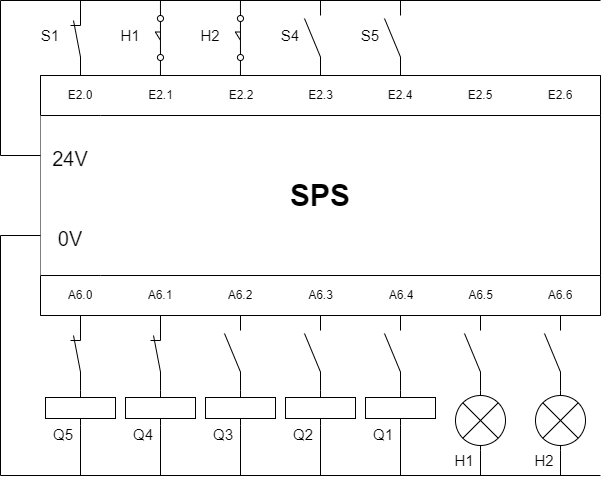
\includegraphics[width=0.8\textwidth]{./images/Anschlussschema.png}
    \caption[Anschlussschema der SPS]{Anschlussschema der SPS}
\end{figure}

### Human Machine Interface (HMI)

Es gibt in jeder Etage, in die der Lastenlift fährt, einen Druckknopf. Dieser Knopf ist dazu da, um den Lift zu rufen und die Türen zu öffnen. Im Lift gibt es zwei Druckknöpfe, wobei einer dafür dient, um in den unteren Stock zu fahren. Der andere dient dazu, um in den oberen Stock zu fahren. Zudem können mit den Knöpfen die Türen geöffnet werden. Im folgendem Bild werden alle Endschalter, Sensoren, Leuchten und Stockwerke abgebildet.

- hS1 und hS2 stellen Lampen dar _(sie zeigen an, in welcher Etage sich der Lift befindet)_
- SEndS1 und SEndS2 stellen den unteren und oberen Endschalter dar _(sie erkennen, ob der Lift im unteren oder oberen Stockwerk angekommen ist)_
- sMoveToS1 und sMoveToS2 stellen Taster im Lift dar _(sie werden zur Navigation des Liftes verwendet)_
- sSendToS1 und sSendToS2 stellen Taster außerhalb des Liftes dar _(sie werden zum Rufen des Liftes verwendet)_
- sDoorBlock stellt den Lichtschacht dar _(dieser wird benötigt, um die Türen zu stoppen, falls diese blockiert wird)_ 
- aDoorS2 und aDoorS1 stellen die jeweiligen Türen in den Stockwerken dar
- aDoorElev stellt die Lifttür dar

\begin{figure}[H]
    \centering
    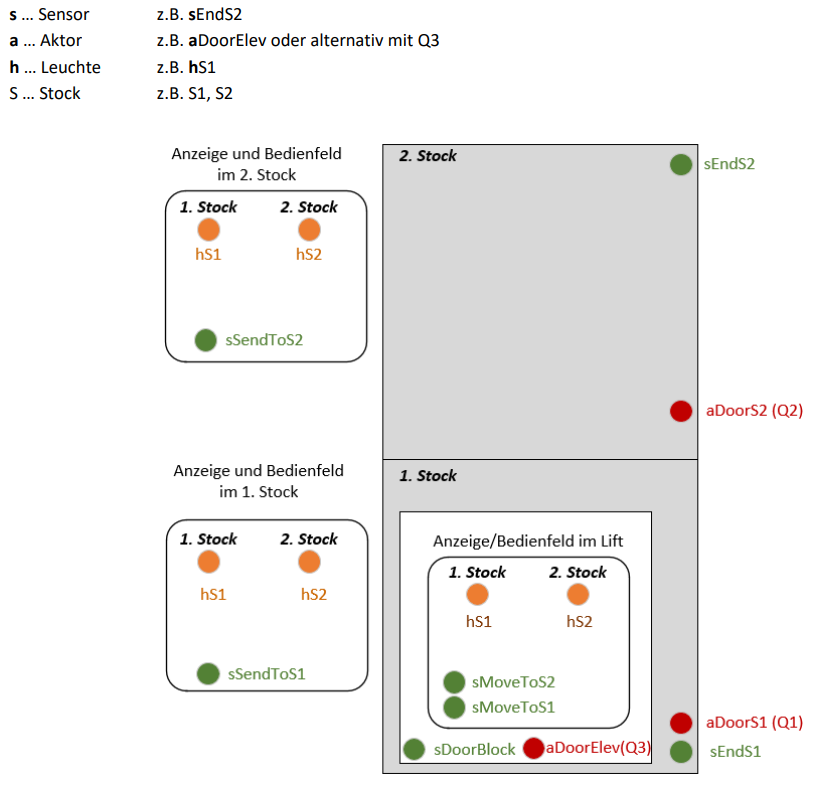
\includegraphics[width=0.8\textwidth]{./images/Skizze.png}
    \caption[Skizze des Lastenliftes]{Skizze des Lastenliftes mit Sensoren, Aktoren und Signalleuchten}
\end{figure}

Alle Zustände und Zusammenhänge können aus der folgenden Zustands- und Zuordnungstabelle abgelesen werden:

\begin{figure}[H]
    \centering
    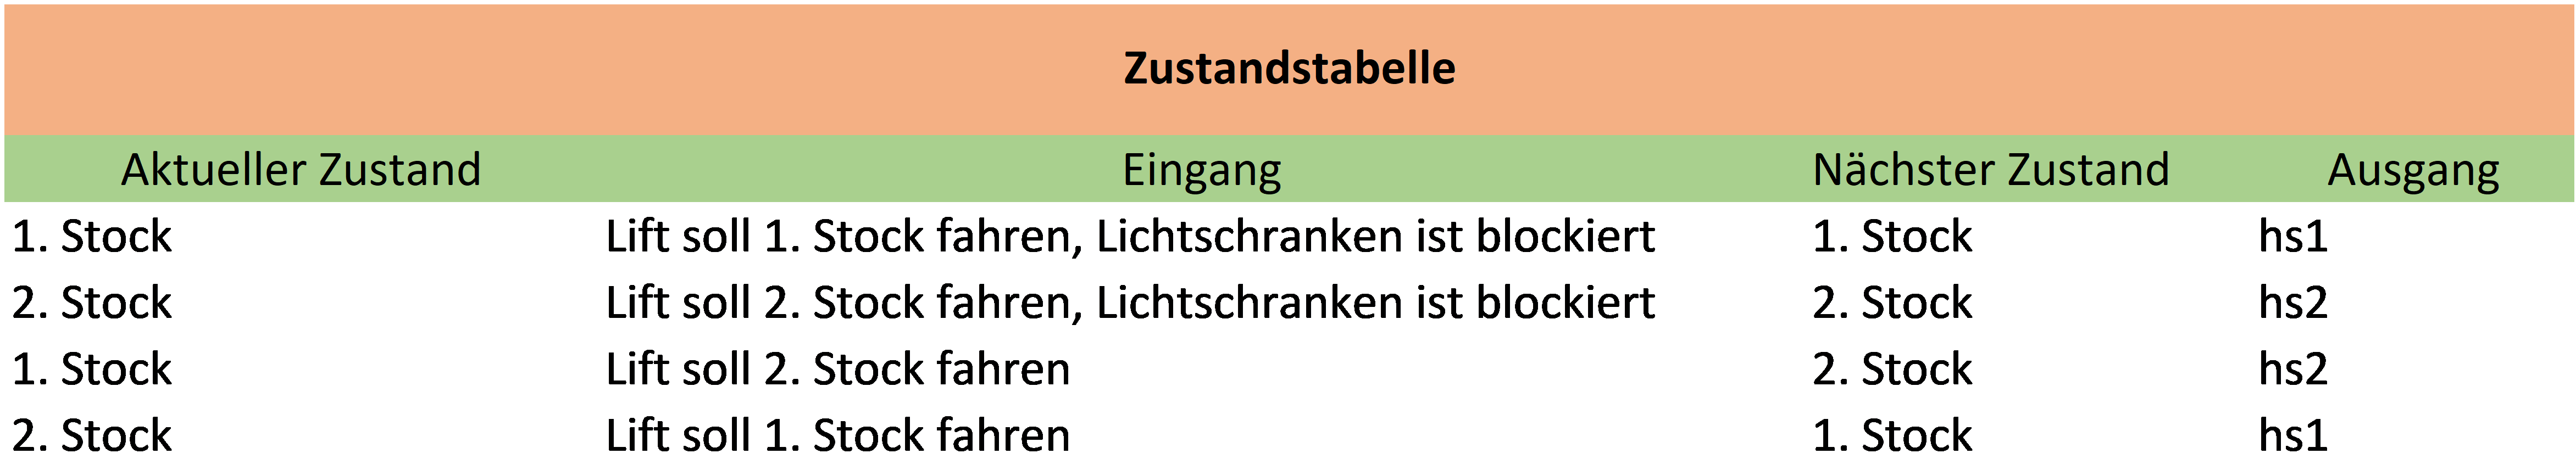
\includegraphics[width=0.8\textwidth]{./images/Zustandstabelle.png}
    \caption[Zustandstabelle]{Zustandstabelle}
\end{figure}

\begin{figure}[H]
    \centering
    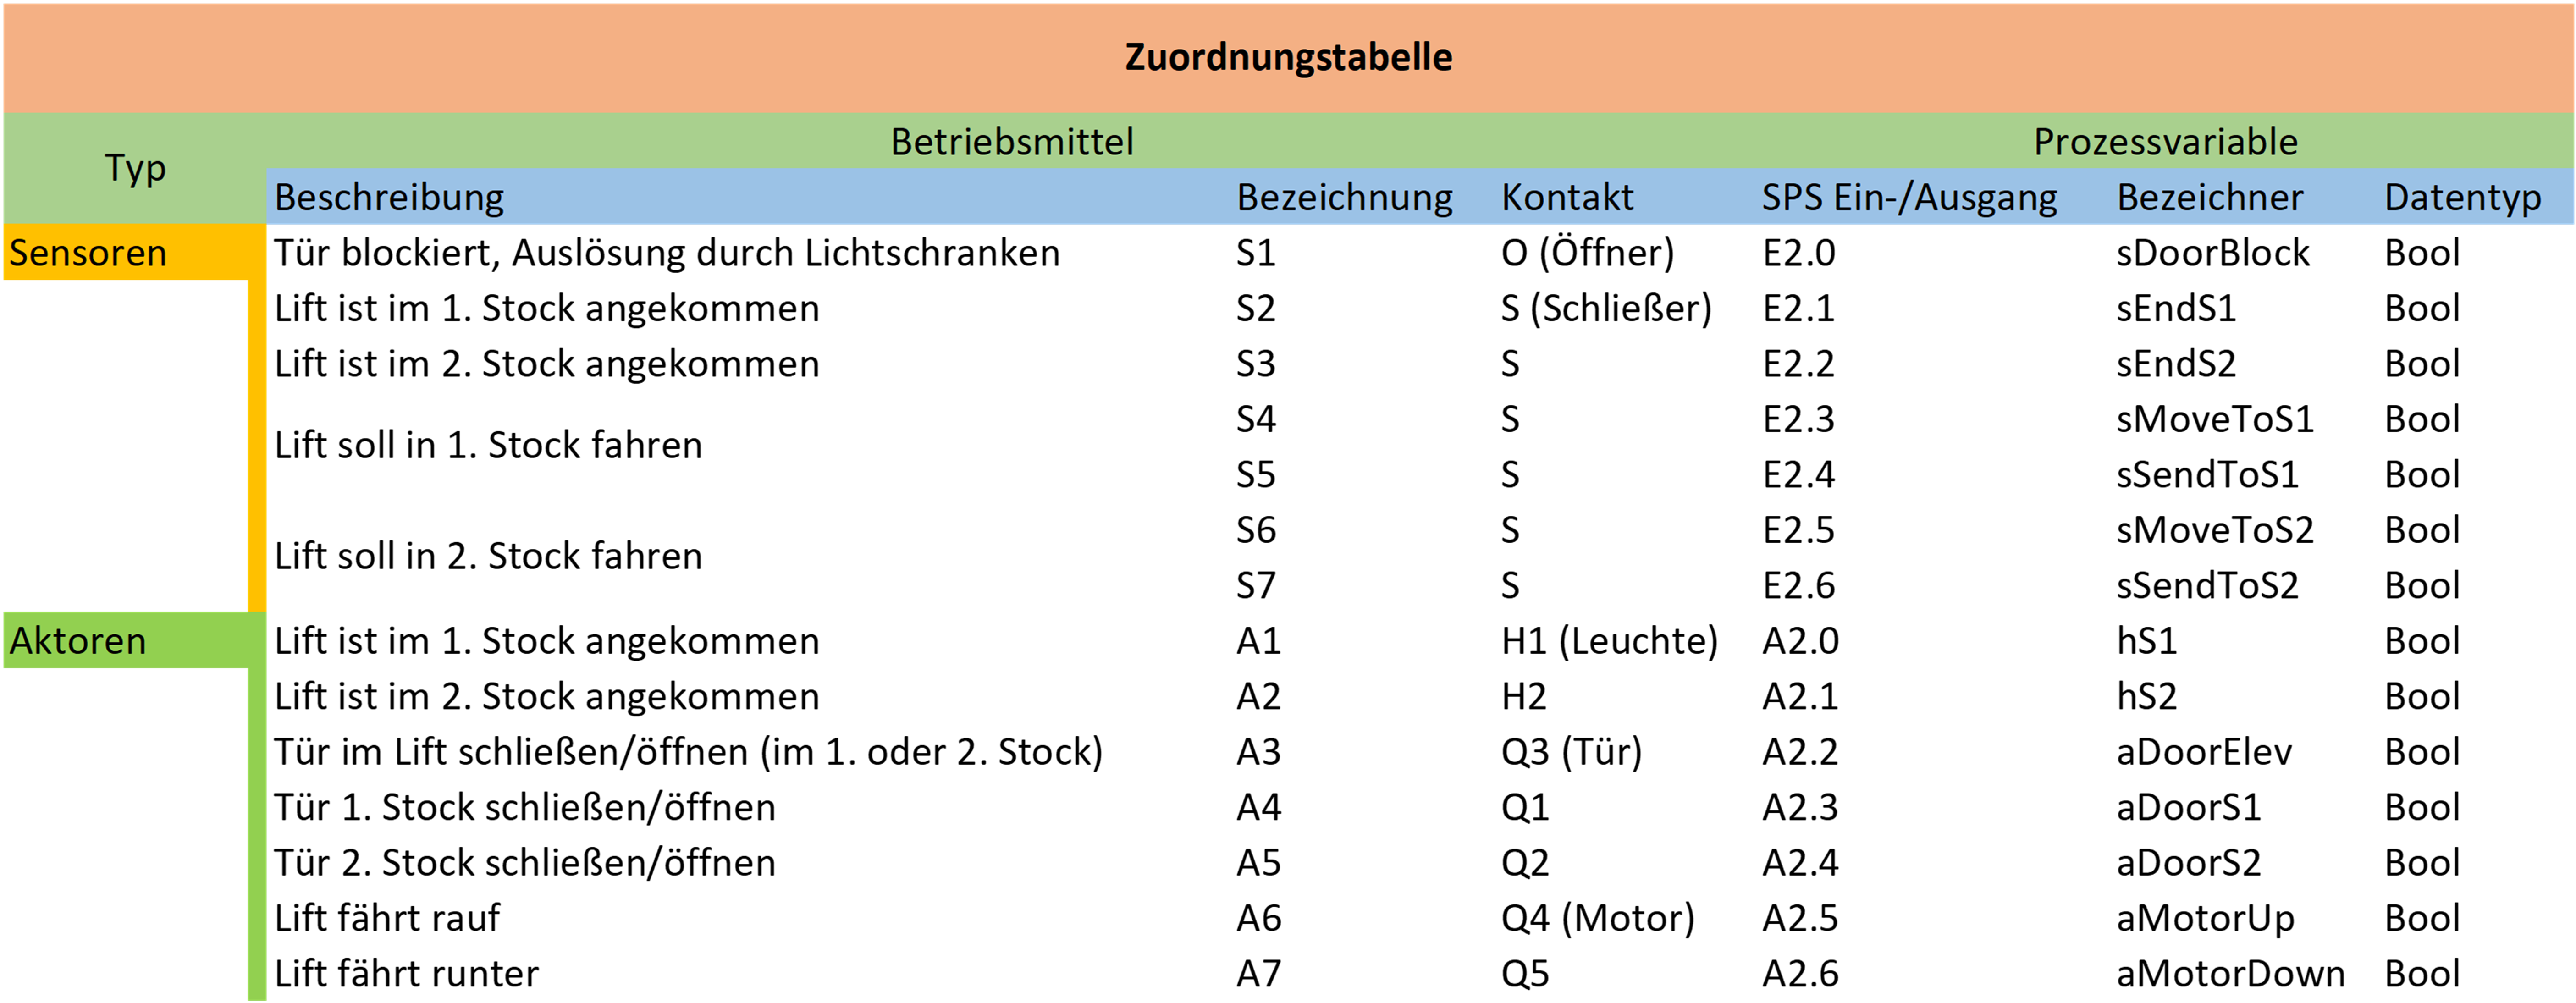
\includegraphics[width=\textwidth]{./images/Zuordnungstabelle.png}
    \caption[Zuordnungstabelle]{Zuordnungstabelle}
\end{figure}

## Softwarespezifikation

Das Programm wird in Automation Studio mit Hilfe von STL (Strukturiertem Text) programmiert. Es wird auf Basis von States umgesetzt. Zudem werden Timer benötigt, um die Lifttüren zeitbasiert zu schließen. Zudem müssen sich, wenn die Lichtschranke blockiert wird, die Lifttüren öffnen, da es sonst zu Sicherheitsrisiken kommen kann. 

### Human Machine Interface (HMI)

Der Lift wird im Einzelschrittbetrieb betrieben und kann nur unter bestimmten Situationen in einen anderen Betriebsmodus wechseln, wie zum Beispiel bei Wartungsarbeiten.

## Test und Industrialisierung

Für alle Sensoren und Aktoren wurden technisch hochwertige Produkte ausgewählt, um die Sicherheit und die Funktionalität zu gewährleisten. Um sicher zu stellen, dass es nach der Inbetriebnahme zu keinerlei Störungen kommt, wurde ein maximales Gewicht festgelegt, welches der Lift befördern darf.

## Maschinensicherheit

Um den Lift in Betrieb nehmen zu dürfen, ist ein CE-Kennzeichen von Nöten. Deshalb müssen alle notwendigen Normen eingehalten werden.
\end{markdown}
%\end{noindent}
\section{Erweiterte Ziel- oder Wunschkriterien}

Es wäre möglich, einen Sensor einzubauen, welcher erkennt wenn der Lift überladen wurde. Zudem währe ein Drucksensor an den Türen sinnvoll. Um eine sanfte abbremsung zu ermöglichen könnten statt den Endschalter, optische Abstandssensoren verbaut werden.
\input{src/05-Geräteaufbau.tex}

\clearpage
\section{Aufwände}

\subsection{Zeitliche Meilensteine in der Projektabwicklung}

\begin{HistoryTimeline}[Meilensteine]
    \HistoryTlEntry{2022-05-05}{\#1}{Rene Hampölz}{Zuordnungstabelle Sensoren/Aktoren}
    \HistoryTlEntry{2022-05-12}{\#2}{Rene Hampölz}{Auswahl der Sensorik}
    \HistoryTlEntry{2022-05-23}{\#3}{Rene Hampölz}{Anschlussschema für die SPS}
    \HistoryTlEntry{2022-06-09}{\#4}{Rene Hampölz}{Programmierung mit Automation Studio}
    \HistoryTlEntry{2022-06-23}{\#5}{Rene Hampölz}{Visualisierung}
\end{HistoryTimeline}

\subsection{Finanzielle Aufwendungen}

In der Tabelle unterhalb werden die Kosten für die Endschalter und für den Lichtvorhang aufgelistet.

%\begin{noindent}
\begin{markdown}

\begin{center}

| Anzahl | Name          | Bezugsquelle          | Kosten  |
|--------|---------------|-----------------------|---------|
| 2x     | AT4/11-3/I/AR | EATON                 | 311,50€ |
| 1x     | DeTec2 Core   | Telco Sensors Austria | 435,24€ |

\end{center}

\end{markdown}
%\end{noindent}

\clearpage

% \clearpage
% 
% \nocite{*}
% \printbibliography

\IncludeHistoryTable

\end{document}